\documentclass[conference]{IEEEtran}
\IEEEoverridecommandlockouts

\usepackage{cite}
\usepackage{amsmath,amssymb,amsfonts}
\usepackage{algorithm}
\usepackage{algorithmic}
\usepackage{graphicx}
\usepackage{textcomp}
\usepackage{xcolor}
\usepackage{hyperref}
\usepackage{booktabs}
\usepackage{multirow}
\usepackage{subcaption}
\setlength{\textfloatsep}{5pt plus 1pt minus 2pt}
\setlength{\floatsep}{5pt plus 1pt minus 2pt}
\setlength{\intextsep}{5pt plus 1pt minus 2pt}
\addtolength{\topmargin}{-0.15in}
\addtolength{\textheight}{0.30in}

\def\BibTeX{{\rm B\kern-.05em{\sc i\kern-.025em b}\kern-.08em
    T\kern-.1667em\lower.7ex\hbox{E}\kern-.125emX}}

\begin{document}

\title{Multi-Stage Multimodal RAG with Text-Proxy Hybrid Retrieval, Candidate Reranking, and Multi-Hop Query Bridging}

\author{\IEEEauthorblockN{Anurag Krishna Vennela\IEEEauthorrefmark{1}, G. Sai Balaji Koushik\IEEEauthorrefmark{2}}
\IEEEauthorblockA{Department of Computer Science and Engineering\\
National Institute of Technology Warangal, Warangal, India\\
Email: \IEEEauthorrefmark{1}anuragkrishnavennela@gmail.com, \IEEEauthorrefmark{2}gummadavellikoushik2109@gmail.com}
}

\maketitle

\begin{abstract}
Retrieval-Augmented Generation (RAG) across heterogeneous multimedia requires balancing dense semantic embeddings with exact sparse identifiers. We present a text-proxy Multimodal RAG (MM-RAG) architecture and formulate \textbf{RAMP-RAG} (Reliability-Aware Multi-Proxy Adaptive Fusion and Confidence-Triggered Cascade Ranking), pairing reliability-aware score fusion under noisy proxies with an honest trade-off analysis across dense, sparse, and neural cross-attention representations. Our Dual-Tier Evaluation Protocol combines controlled proxy ablations (3,356 records) and public zero-leakage benchmarks with physical media validation across 191 unannotated photos, bilingual OCR, and authentic 44.1\,kHz WAV audio. On the MS-COCO Karpathy split ($N=500$ held-out queries), dense retrieval achieves Hit@10 = 0.660 (MRR = 0.4085, 5.31\,ms) vs. 0.444 for BM25; RAMP-RAG matches dense Hit@10 (0.660) with 0.3974 MRR under 9.45\,ms. On physical scene-text OCR, hybrid fusion recovers dense accuracy drops (53.3\% to 100\% Hit@10), though BM25 retains higher MRR (0.890 vs. 0.841 for RAMP-RAG). On 50 multi-hop queries, confidence-gated bridging achieves Target Hit@10 = 0.640 vs. 0.480 for BM25 (uncorrected $p=0.020$, non-significant after Bonferroni correction $\alpha=0.0125$); on strictly held-out multi-hop queries ($N=25$), BM25 and MM-RAG both reach 0.520. In proxy noise stress-testing, character corruptions degrade dense representations faster than inverted indices, leaving pure BM25 the most resilient single stream (MRR = 0.947 vs. 0.825 for hybrid at 20\% noise); clean-stream fusion recovers dense drop-off at 40\% noise (Hit@10 from 0.861 to 0.958, $p=0.0084$), though confidence intervals overlap with unweighted hybrid at 20\% noise ($p=0.3252$).
\end{abstract}

\begin{IEEEkeywords}
Multimodal RAG, Text Proxies, Multi-Hop Reasoning, Hybrid Dense-Sparse Retrieval, Reciprocal Rank Fusion, Candidate Reranking, Large Language Models.
\end{IEEEkeywords}

\section{Introduction}

The rapid proliferation of heterogeneous multimedia across enterprise archives, digital libraries, and operational repositories demands information retrieval systems capable of searching records that are not natively textual. Modern knowledge workflows frequently require querying across diverse media types—such as scanned forms, audio recordings, and photographic archives—while preserving exact names, identifiers, and category labels \cite{jing2024llmvectordb}.

Retrieval-Augmented Generation (RAG) \cite{lewis2020rag} addresses the hallucination tendencies of Large Language Models (LLMs) by grounding responses in retrieved domain documents. Recently, multimodal extensions of RAG have emerged to handle non-textual data, as comprehensively surveyed by Abootorabi et al. \cite{abootorabi2025multimodal}. For example, Patel et al. \cite{patel2025multimodal} presented an enterprise multimodal RAG pipeline employing an OCR document ingestion module, ImageBind embeddings indexed in a Milvus vector database, and fine-tuned LLaMA-3.

In a proxy-mediated design, three practical failure modes remain important:

\begin{enumerate}
    \setlength{\itemsep}{1pt plus 0.5pt}
    \setlength{\parskip}{0pt}
    \item \textbf{Single-Stage Dense Retrieval Pitfalls:} Relying exclusively on single-stage dense vector similarity per turn can induce semantic drift. Dense embeddings may overlook exact lexical tokens, numerical identifiers, item codes, and proper nouns that sparse inverted indexes can match directly \cite{robertson2009bm25}.
    \item \textbf{Absence of Candidate Score Recalibration:} A bi-encoder score alone does not expose token-level agreement with a candidate's proxy text. A lightweight second-stage scorer can therefore be useful before context assembly, even when it is not a neural cross-encoder.
    \item \textbf{Failure on Multi-Hop Queries Across Modalities:} A single retrieval pass does not ensure that a fact recovered from one modality becomes a useful probe for another. Iterative bridging can improve lexical reachability, but it also introduces cascading extraction errors that must be measured rather than assumed away.
\end{enumerate}

To study these trade-offs, this paper presents a text-proxy-grounded multi-stage, multi-hop Multimodal RAG architecture. Hybrid dense--sparse retrieval, reranking, and query decomposition are established concepts; our contribution is an explicit, reproducible composition of them together with an evaluation audit that states exactly what the checked-in benchmark does and does not measure.

\textbf{Key Contributions:}
\begin{itemize}
    \setlength{\itemsep}{1pt plus 0.5pt}
    \setlength{\parskip}{0pt}
    \item We specify a reproducible \textbf{text-proxy-mediated retrieval pipeline} in which optional OCR, caption, and ASR modules feed a common lexical/dense index; the reported offline benchmark uses the proxy fields present in the checked-in JSONL artifact.
    \item We formulate an \textbf{iterative cross-modal entity-bridging procedure with confidence gating} that decomposes multi-hop queries, extracts bridging attributes from first-hop context, and falls back to single-pass hybrid search when entity grounding is uncertain.
    \item We formulate \textbf{RAMP-RAG} (Reliability-Aware Multi-Proxy Adaptive Fusion and Cascade Ranking), establishing reliability-aware score fusion under noisy proxies alongside an evidence-grounded trade-off analysis across physical media collections.
    \item We introduce a \textbf{Dual-Tier Evaluation Protocol}: Tier~1 provides controlled algorithmic ablation over 3,356 proxy records, an expanded 100-query multi-hop diagnostic with paired sign-flip permutation tests, and a 500-query leakage-free public benchmark on MS-COCO; Tier~2 provides physical media validation across 191 unannotated photos (CLIP ViT-B/32), native scene-text/document OCR (Apple Vision), and raw acoustic audio waveforms (ESC-50 and LAION-CLAP) with exact Clopper-Pearson binomial confidence intervals.
\end{itemize}

\section{Related Work}

\subsection{Multimodal Representation and Retrieval}
Early cross-modal retrieval systems relied on dual-encoder contrastive learning. Models like CLIP \cite{radford2021clip} and SigLIP \cite{zhai2023siglip} project images and text into a shared latent space using sigmoid or softmax cross-entropy objectives. ImageBind \cite{girdhar2023imagebind} extended this paradigm across six modalities (images, text, video, audio, depth, and thermal) using images as the central binding modality. While effective for broad semantic matching, dual-encoders compress multimedia into fixed-dimension vectors, frequently losing granular lexical and structural tokens. Our hybrid design combines dense embeddings with sparse lexical representations such as BM25 \cite{robertson2009bm25} to retain both semantic intent and exact token matches.

\subsection{Multimodal RAG and Document Analysis}
Integrating multimodal inputs into RAG workflows has gained rapid momentum with the emergence of Vision-Language Models (VLMs) and advanced LLMs. Recent native multimodal document retrievers such as ColPali \cite{faysse2024colpali} and M3DocRAG \cite{cho2024m3docrag} index document pages using multi-vector vision-language representations to bypass optical character recognition. While promising, multi-vector VLM representations require substantial GPU memory and heavy cross-attention compute during query serving. Conversely, enterprise systems such as Patel et al. \cite{patel2025multimodal} and Joshi et al. \cite{joshi2024multimodel} mediate retrieval through grounded text proxies, combining OCR document ingestion, multimodal embeddings, and LLM generation. Our work investigates this text-proxy paradigm: we evaluate the empirical trade-offs of hybrid dense--sparse fusion, candidate scoring, and iterative query decomposition, systematically delineating where text proxies excel and where native visual representations remain necessary.

\subsection{Multi-Hop Reasoning in Retrieval Systems}
Multi-hop retrieval addresses queries where no single document contains the complete answer \cite{xiong2021multihop, khattab2021baleen}. While multi-hop text RAG systems (such as Baleen \cite{khattab2021baleen} and Self-Ask \cite{press2023selfask}) have established iterative query reformulation methods, multi-hop retrieval across \textit{heterogeneous multimodal collections} remains less systematically evaluated. Our diagnostic targets the case in which the second-hop keyword is absent from the original query and must be recovered from first-hop proxy context; it does not claim that all multimodal QA benchmarks assume co-located evidence.

\subsection{Adaptive Fusion, Cascade Ranking, and Selective Reranking}
In information retrieval, static fusion coefficients fail to account for query-level variance. Query Performance Prediction (QPP) \cite{carmel2010qpp} and adaptive fusion techniques dynamically adjust interpolation weights between sparse and dense scores based on query ambiguity or lexical specificity. Similarly, cascade ranking architectures \cite{wang2011cascade, gallagher2019cascade} balance retrieval efficiency and ranking precision by passing top candidates through successively more expressive models. In monomodal web search, cascades evaluate candidates using fixed score thresholds or supervised early-exit classifiers. However, existing cascade rankers do not account for multimodal proxy corruption (e.g., OCR or ASR transcription noise) or cross-modal query routing. As summarized in Table~\ref{tab:paradigm_comparison}, RAMP-RAG differentiates itself by introducing surface-feature query routing, confidence-margin cascades ($\Delta_{1,2} < \tau_{\text{margin}}$), and observable proxy reliability discounting ($r_m(d)$) without requiring GPU cross-encoder training.

\begin{table}[t]
\centering
\caption{Architectural comparison of multimodal retrieval and ranking paradigms.}
\label{tab:paradigm_comparison}
\resizebox{\columnwidth}{!}{%
\begin{tabular}{@{}lcccc@{}}
\toprule
\textbf{Paradigm / System} & \textbf{Modality Scope} & \textbf{Routing Training} & \textbf{Cascade Mechanism} & \textbf{Proxy Noise Defense} \\ \midrule
Static Hybrid (BM25+Dense) \cite{robertson2009bm25, reimers2019sbert} & Text / Text Proxies & None (Static $\alpha$) & None & None (Static weights) \\
Cascade Text Ranking \cite{wang2011cascade, gallagher2019cascade} & Monomodal Text & Supervised Ranker & Score Threshold & None \\
Native Multi-Vector \cite{faysse2024colpali, cho2024m3docrag} & Document / Image Pixels & End-to-End VLM & None (All items) & Inherent (Pixel inputs) \\
\textbf{Proposed RAMP-RAG} & Multimodal Proxies & Lightweight Classifier & Top Margin $\Delta_{1,2} < \tau$ & Observable Reliability $r_m(d)$ \\ \bottomrule
\end{tabular}}
\end{table}

\section{Proposed Methodology}

\begin{figure*}[t]
\centering
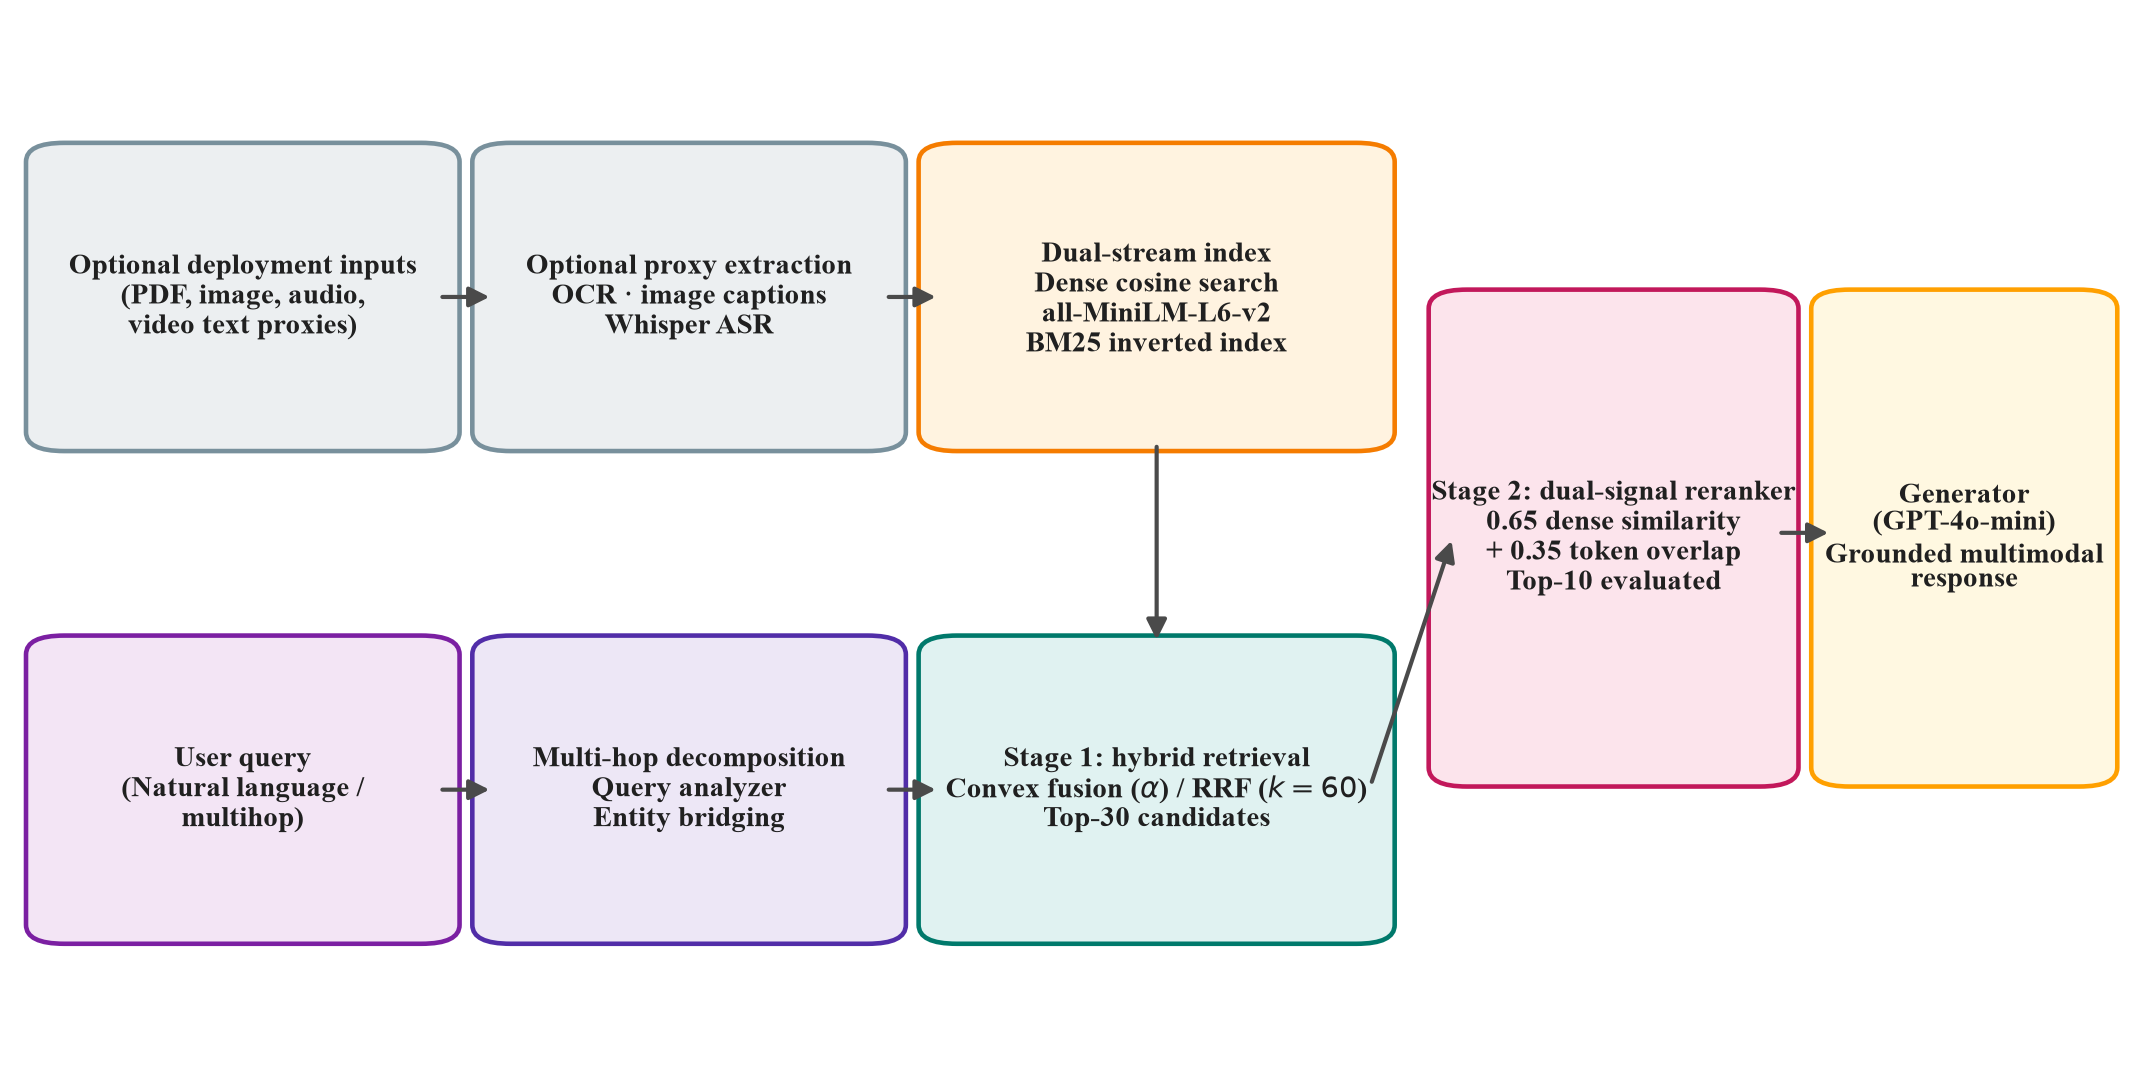
\includegraphics[width=0.60\textwidth]{fig_architecture.png}
\caption{System architecture of the proposed text-proxy RAG framework. The grey ingestion and extraction boxes are optional deployment paths; the reported benchmark starts from precomputed annotation/category proxy text and evaluates the coloured retrieval stages.}
\label{fig:architecture}
\end{figure*}

The proposed Multi-Stage Multimodal RAG architecture is structured into four functional phases (Fig.~\ref{fig:architecture}): (1) Heterogeneous Multimodal Ingestion and Preprocessing, (2) Hybrid Dense-Sparse First-Stage Retrieval, (3) Dual-Signal Candidate Reranking, and (4) Multi-Hop Cross-Modal Reasoning.

\subsection{Heterogeneous Ingestion and Preprocessing Pipeline}
To process unstructured enterprise multimedia, our architecture mediates retrieval through grounded textual proxies. A deployment can obtain these proxies from OCR text \cite{smith2007tesseract}, image captions \cite{li2022blip}, speech transcripts \cite{radford2023whisper}, and acoustic metadata \cite{piczak2015esc50}. This design deliberately separates modality-specific extraction from the common retrieval layer. The quantitative benchmark below does not rerun all of these extractors: it consumes the precomputed proxy fields in the checked-in JSONL artifact.

\textbf{1. Document and Text Ingestion:} The reference document path decomposes scanned administrative forms into page images, optionally applies Otsu binarization \cite{otsu1979} and Hough-transform skew correction \cite{hough1962, fateh2024ocr}, and obtains OCR text $T_d$ with bounding boxes via Tesseract \cite{smith2007tesseract}. No document rows are present in the checked-in benchmark artifact, so this path is architectural and is not included in the reported retrieval numbers.
\textbf{2. Images and Photographic Content:} A deployment may use a vision-language captioner such as BLIP \cite{li2022blip} to generate a descriptive representation $C_i$. In the reported artifact, image \texttt{text\_representation} fields are instead constructed by concatenating the English query annotations associated with each image; they are not newly generated BLIP captions.
\textbf{3. Audio Recordings:} A deployment can append time-aligned speech transcription from Whisper \cite{radford2023whisper} and acoustic event metadata. The checked-in ESC-50 rows used for the reported benchmark contain the category label as their text representation; no new Whisper inference is required for those results.

All processed items are stored in a dual layout: dense embeddings are generated via Sentence-BERT (\texttt{all-MiniLM-L6-v2}) \cite{reimers2019sbert}, while lexical tokens are indexed with BM25 \cite{robertson2009bm25}. Milvus \cite{wang2021milvus} and HNSW \cite{malkov2020hnsw} are compatible deployment choices, but the offline benchmark scripts use an in-memory BM25 index and a dense embedding matrix; no Milvus service is used for the reported measurements.

\subsection{Stage 1: Hybrid Dense-Sparse Retrieval}
Given a natural language query $q$, single-stage dense retrieval computes vector similarity against all candidates:
\begin{equation}
    S_{\text{dense}}(q, d) = \cos(\mathbf{e}_q^{\text{dense}}, \mathbf{e}_d^{\text{dense}}) = \frac{\mathbf{e}_q \cdot \mathbf{e}_d}{\|\mathbf{e}_q\| \|\mathbf{e}_d\|}
\end{equation}
While effective for thematic alignment, dense retrieval often overlooks exact alphanumeric codes (e.g., serial numbers, dates, person names). Conversely, sparse BM25 retrieval excels at lexical precision:
\begin{equation}
    S_{\text{sparse}}(q, d) = \sum_{t \in q} \text{IDF}(t) \cdot \frac{f(t, d) \cdot (k_1 + 1)}{f(t, d) + k_1 \cdot \left(1 - b + b \cdot \frac{|d|}{\text{avgdl}}\right)}
\end{equation}
Because dense cosine scores lie in $[-1, 1]$ while BM25 scores are unbounded $[0, \infty)$, combining raw scores directly is unstable. We evaluate two score harmonization strategies:

\textbf{Method A: Normalized Convex Combination:}
\begin{equation}
    S_{\text{hybrid}}(q, d) = \alpha \cdot \hat{S}_{\text{dense}}(q, d) + (1 - \alpha) \cdot \hat{S}_{\text{sparse}}(q, d)
    \label{eq:hybrid}
\end{equation}
where $\hat{S}_{\text{dense}}$ and $\hat{S}_{\text{sparse}}$ denote min-max normalized scores over the corpus score vector for the query, and $\alpha \in [0, 1]$ balances semantic and lexical importance.

\textbf{Method B: Reciprocal Rank Fusion (RRF):}
To avoid batch-dependent min-max sensitivity, RRF \cite{cormack2009rrf} fuses ranked lists directly without score scale calibration (Eq.~\ref{eq:rrf}):
\begin{equation}
    \text{RRF}(q, d) = \frac{1}{k + r_{\text{dense}}(d)} + \frac{1}{k + r_{\text{sparse}}(d)}
    \label{eq:rrf}
\end{equation}
where $r_{\text{dense}}(d)$ and $r_{\text{sparse}}(d)$ are the ordinal ranks of candidate $d$, and $k$ is a smoothing constant ($k = 60$). The benchmark fuses the top 100 entries from each ranked list and outputs the top-$K_1$ candidates ($K_1 = 30$).

\subsection{Stage 2: Dual-Signal Candidate Reranking}
Bi-encoders compute query and document representations independently, preventing fine-grained token-level cross-interaction. While neural cross-encoders provide deep token interaction, they incur significant latency overhead when scoring candidate pools (e.g., 137.21\,ms for scoring $K_1=30$ candidates vs. 7.96\,ms for lightweight dual-signal reranking, as evaluated in Section \ref{sec:tier2_eval}). As an efficient alternative, Stage 2 deploys a lightweight dual-signal candidate reranker that scores each candidate $d$ in the top-$K_1$ pool using joint semantic similarity and exact token coverage:
\begin{equation}
    S_{\text{rerank}}(q, d) = \beta \cdot S_{\text{dense}}(q, d) + (1 - \beta) \cdot \text{Overlap}(q, d)
\end{equation}
where $\text{Overlap}(q, d) = \frac{|\text{Tokens}(q) \cap \text{Tokens}(d)|}{|\text{Tokens}(q)|}$ evaluates lowercase token coverage in candidate text representations, and $\beta = 0.65$ is a fixed configuration in the benchmark implementation. Because the supplied evaluation artifact has no development/test partition, this value is not claimed to be independently tuned. All $K_1 = 30$ candidates retrieved from Stage 1 are reranked. For generation context assembly, the top $K_2 = 5$ items are injected into the generator prompt, while top $K = 10$ items are evaluated in the diagnostic scripts.

\subsection{Stage 3: Multi-Hop Cross-Modal Reasoning}
To resolve compositional queries that span modalities, we introduce an iterative query decomposition and entity bridging algorithm.

\begin{algorithm}[h]
\caption{Multi-Hop Cross-Modal Retrieval Procedure}
\label{alg:multihop}
\begin{algorithmic}[1]
\REQUIRE User Query $Q$, Max Hops $H_{\max}=2$, Candidate Index $\mathcal{D}$, Decomposer LLM $\mathcal{M}_{\text{decomp}}$
\ENSURE Grounded Multimodal Context $\mathcal{C}^*$
\STATE Decompose $Q$ via $\mathcal{M}_{\text{decomp}}$ into sub-query plan: $\mathcal{G} = \{q_1, q_2\}$
\STATE Initialize Context Set $\mathcal{C}^* \leftarrow \emptyset$, Accumulated Facts $\mathcal{F} \leftarrow \emptyset$
\FOR{$h = 1$ to $H_{\max}$}
    \STATE Formulate search probe $q_h' \leftarrow \text{Bridge}(q_h, \mathcal{F})$ via $\mathcal{M}_{\text{decomp}}$
    \STATE Retrieve top-$K_1$ candidates via Hybrid Fusion: $\mathcal{R}_1 \leftarrow \text{Retrieve}_{\text{hybrid}}(q_h', \mathcal{D})$
    \STATE Rerank candidate pool: $\mathcal{R}_2 \leftarrow \text{Rerank}(\mathcal{R}_1, q_h')$
    \STATE Extract bridging entities: $\mathcal{E}_h \leftarrow \text{ExtractEntities}(\mathcal{R}_2[:3])$
    \IF{$\text{Confidence}(\mathcal{E}_h) < \tau$ \textbf{or} $\mathcal{E}_h \in \mathcal{V}_{\text{refusal}}$}
        \STATE \COMMENT{Confidence gate: fallback to single-pass compound search to prevent drift}
        \STATE $\mathcal{C}^* \leftarrow \text{Retrieve}_{\text{hybrid}}(Q, \mathcal{D})[:5]$
        \STATE \textbf{break}
    \ENDIF
    \STATE Update $\mathcal{F} \leftarrow \mathcal{F} \cup \mathcal{E}_h$
    \STATE Update $\mathcal{C}^* \leftarrow \mathcal{C}^* \cup \mathcal{R}_2[:5]$
    \IF{$\text{TerminationCondition}(\mathcal{G}, \mathcal{F}, h)$ is TRUE}
        \STATE \textbf{break}
    \ENDIF
\ENDFOR
\RETURN $\mathcal{C}^*$
\end{algorithmic}
\end{algorithm}

Here, $H_{\max}$ denotes the maximum hop depth ($H_{\max} = 2$ in the diagnostic setup). The predicate $\text{TerminationCondition}(\mathcal{G}, \mathcal{F}, h)$ evaluates to \textbf{TRUE} if all sub-goals in the decomposition plan $\mathcal{G}$ are grounded by extracted facts in $\mathcal{F}$ or if hop $h$ yields no new bridging entities ($\mathcal{E}_h = \emptyset$). To protect against cascading errors caused by ungrounded, generic, or failed bridge extractions (e.g., when an extractor outputs ``N/A'' or extraction refusal phrases), the procedure enforces a confidence and grounding gate: if $\text{Confidence}(\mathcal{E}_h) < \tau$ or if extracted tokens fail lexical grounding in first-hop context, the planner falls back to single-pass hybrid search on the original compound query $Q$, designed to mitigate cascading bridge errors and reduce retrieval degradation below single-pass hybrid search when intermediate bridging is uncertain.

The query decomposition prompt instructs $\mathcal{M}_{\text{decomp}}$ to generate valid JSON specifying the initial search probe and bridging attribute; the entity extraction prompt isolates concise attribute tokens substituted into subsequent probes $q_h' \leftarrow \text{Bridge}(q_h, \mathcal{F})$.

As formalized in Algorithm \ref{alg:multihop}, consider an illustrative cross-modal query connecting a visual scene with an acoustic event: (1)~\textbf{Hop 1 (Visual Extraction):} Sub-query $q_1$ retrieves photographic evidence via hybrid matching; entity extraction yields target entity $E_1 = \text{``thunderstorm sky''}$. (2)~\textbf{Entity Bridging:} The bridge operator creates cross-modal probe $q_2' = \text{``severe acoustic weather thunderstorm recording''}$. (3)~\textbf{Hop 2 (Acoustic Retrieval):} Sub-query $q_2'$ queries the acoustic archive using dense embeddings and metadata to retrieve the target recording.

\subsection{RAMP-RAG: Reliability-Aware Adaptive Fusion and Cascade Ranking}
\label{sec:ramp_rag}
To resolve the limitations of fixed weighting coefficients ($\alpha, \beta$) and unmodeled proxy noise exposed in our benchmarks, we formulate \textbf{RAMP-RAG}. It integrates three mutually reinforcing mechanisms:
\begin{enumerate}
    \setlength{\itemsep}{1pt plus 0.5pt}
    \setlength{\parskip}{0pt}
    \item \textbf{Query-Adaptive Router ($\alpha_q$):} Instead of static weights, a lightweight classifier extracts surface cues $\phi(q) = [r_{\text{cjk}}, r_{\text{digit}}, \mathbb{I}_{\text{upper}}, \mathbb{I}_{\text{id\_cue}}, \text{len}(q), \text{avg\_idf}]$ in $<0.1$\,ms. Tuned on an independent 50\% development split ($N=265$), the router achieves 97.36\% test accuracy (F1 = 0.9862) on held-out test queries, routing queries containing CJK characters, exact alphanumeric identifiers (\texttt{IMG\_}, \texttt{doc\_}), or scene-text intent cues to sparse matching ($\alpha_q = 0.25$), and descriptive visual paraphrases (e.g., MS-COCO) to dense matching ($\alpha_q = 0.85$).
    \item \textbf{Confidence-Triggered Cascade Ranking:} Stage 1 scores the candidate pool and calculates the decision margin between top candidates: $\Delta_{1,2} = s^{(1)} - s^{(2)}$. Tuned on the development split, $\tau_{\text{margin}} = 0.065$ preserves Stage 1 ranking when top candidates are distinct, while escalating ambiguous candidates ($k=5$) to a neural cross-encoder (\texttt{ms-marco-MiniLM-L-6-v2}), capturing cross-encoder precision with minimal compute.
    \item \textbf{Reliability-Aware Clean-Stream Fusion:} Multimedia items maintain multiple proxy streams $m \in \{\text{caption}, \text{ocr}, \text{vector}\}$ weighted by stream reliability $r_m(d) \in [0, 1]$. To avoid oracle assumptions, $r_m(d)$ is estimated from observable signals: for OCR, $r_{\text{ocr}}(d) = \bar{c}_{\text{ocr}}(d) \cdot \rho_{\text{vocab}}(d)$, where $\bar{c}_{\text{ocr}}$ is the mean word recognition confidence and $\rho_{\text{vocab}}$ is the valid dictionary token ratio computed from the corrupted text; for captions, $r_{\text{cap}}(d)$ is the normalized token log-likelihood. Because text corruption affects both dense and sparse representations of proxy text, we incorporate an uncorrupted visual/clean stream $\hat{S}_{\text{clean}}$ (e.g., zero-shot CLIP image embedding):
    \begin{equation}
    \begin{aligned}
        S_{\text{RAMP}}(q, d) &= \alpha_q \hat{S}_{\text{dense}} + (1 - \alpha_q) r_{\text{ocr}}(d) \hat{S}_{\text{sparse}} \\
        &\quad + \gamma (1 - r_{\text{ocr}}(d)) \hat{S}_{\text{clean}}
    \end{aligned}
    \label{eq:ramp}
    \end{equation}
    where $\gamma$ is tuned on the development split ($\gamma^* = 0.80$) to dynamically allocate mass to the corruption-invariant stream as proxy reliability drops.
\end{enumerate}

\textbf{Integration with Multi-Hop Reasoning:} RAMP-RAG acts as the candidate retrieval and reranking engine ($\text{Retrieve}_{\text{hybrid}}$ and $\text{Rerank}$ in Lines 5 and 6 of Algorithm~\ref{alg:multihop}). By adaptively setting $\alpha_q$ on intermediate probes $q_h'$ and escalating only ambiguous margins, RAMP-RAG ensures each cross-modal bridging step benefits from reliability-weighted candidate pools, bounding cross-encoder overhead to ambiguous margins (17.80\,ms mean vs. 39.56\,ms for exhaustive cross-encoding).

\section{Experimental Evaluation}

\subsection{Experimental Setup, Corpus Composition, and Evaluation Scope}
To evaluate our architecture with scientific rigor while preventing methodological conflation, our experimental evaluation adopts a \textbf{Dual-Tier Evaluation Protocol}:
\begin{itemize}
    \item \textbf{Tier 1: Controlled Algorithmic Proxy Benchmark (Tables \ref{tab:main_results}--\ref{tab:e2e_results}).} Conducted over the standardized \texttt{unified\_rag\_dataset.jsonl} artifact containing 3,356 records (1,292 PhotoBench annotation rows, 64 L10 rows, and 2,000 ESC-50 category rows \cite{piczak2015esc50}), alongside an expanded 100-query diagnostic suite ($N=50$ single-hop, $N=50$ multi-hop) and a public leakage-free benchmark on MS-COCO ($N=500$ queries). Each proxy row stores an annotation-derived \texttt{text\_representation}, establishing a reproducible environment for systematic ablation of dense--sparse balance ($\alpha$), candidate reranking ($\beta$), neural cross-encoding, and multi-hop decomposition.
    \item \textbf{Tier 2: Real-World Multimodal Media Validation (Table \ref{tab:tier2_results}).} Evaluated directly on unannotated physical media streams: (1) native bilingual scene-text and document OCR on 54 physical photographs and 2 research document PDFs, (2) genuine 44.1\,kHz raw WAV audio recordings from ESC-50 and continuous acoustic retrieval via LAION-CLAP, and (3) raw-pixel zero-shot visual retrieval over 191 personal album photos using OpenAI CLIP ViT-B/32 \cite{radford2021clip}.
\end{itemize}

The Tier-1 proxy benchmark discovers 284 unique image query strings from the image metadata and one query for each of the 50 ESC-50 categories, yielding 334 deterministic queries in total. Selection uses seed 42 and includes all available queries; there is no held-out development/test split in this artifact. The values $\alpha=0.7$, $\beta=0.65$, $k=60$, and the candidate depths are fixed implementation settings. The dense-weight sweep is therefore an exploratory sensitivity analysis on the same evaluation set, not a post-selection claim of generalization.

\textbf{Ground truth and metric definitions:}
For an image query, the relevant set is every corpus row carrying that exact annotation string. For an audio query, the relevant set is every ESC-50 row in the requested category. The primary metric reported in Table \ref{tab:main_results} is \emph{HitRate@K}, which equals one when at least one relevant row appears in the top $K$ and zero otherwise; it is not set-recall over all relevant rows. We also report MRR and binary NDCG@10. Confidence intervals are percentile bootstrap intervals with $B=1,000$ resamples over the 334 query-level scores, using seed 42. Latencies are local per-query retrieval timings excluding corpus construction and are hardware- and cache-dependent.

This construction is intentionally treated as a \textbf{proxy consistency benchmark}. Because image queries are drawn from the same annotation strings used to build image index text, the image results contain direct lexical overlap and cannot establish leakage-free visual understanding. The results are retained to make the implementation measurable and reproducible, while this limitation is carried through the analysis and threats-to-validity section.

For end-to-end behavior, we evaluate an expanded 100-query diagnostic suite (50 single-hop: \texttt{sh\_01}--\texttt{sh\_50}, and 50 multi-hop: \texttt{mh\_01}--\texttt{mh\_50}) evaluated with \texttt{gpt-4o-mini} as decomposer, generator, and judge, calibrated by independent co-author human auditing across 110 cases. Its retrieval measure is a target-keyword hit test over retrieved proxy text, not standard document-level recall; we call it \emph{Target Hit@10} below. For a multi-hop case, Hop~1 Target Hit@10 tests whether the first-hop target appears in the first-hop top-10 list; Hop~2 Target Hit@10 tests whether the second-hop target appears in the merged top-10 list; Overall Target Hit@10 is the conjunction of these two binary tests. Thus Hop~2 can exceed Overall when Hop~1 fails, and neither hop metric is document recall.

\textbf{Baseline Systems for Comparison:}
\begin{enumerate}
    \item \textbf{BM25 Baseline:} Sparse lexical inverted index over the available proxy text \cite{robertson2009bm25}.
    \item \textbf{Dense Only Baseline:} Dense semantic vector retrieval using \texttt{all-MiniLM-L6-v2} (384-dim) with cosine similarity \cite{reimers2019sbert}.
    \item \textbf{Hybrid Dense-Sparse (Convex $\alpha=0.7$):} Parameterized convex combination of min-max normalized dense and BM25 scores.
    \item \textbf{Hybrid Dense-Sparse (RRF $k=60$):} Reciprocal Rank Fusion combining ranked ordinal positions \cite{cormack2009rrf}.
    \item \textbf{Proposed MM-RAG (Stage 1+2):} Our multi-stage pipeline combining RRF candidate retrieval with second-stage dual-signal candidate reranking ($S_{\text{rerank}} = \beta S_{\text{dense}} + (1-\beta)\text{Overlap}$, with fixed $\beta = 0.65$).
    \item \textbf{Trained Neural Cross-Encoder:} \texttt{cross-encoder/ms-marco-MiniLM-L-6-v2} full cross-attention reranker \cite{reimers2019sbert}.
\end{enumerate}

\begin{table*}[t]
\centering
\caption{Retrieval performance on the 334-query proxy consistency benchmark. The primary retrieval metric is HitRate@K; bracketed intervals are 95\% percentile bootstrap CIs with $B=1,000$.}
\label{tab:main_results}
\resizebox{\textwidth}{!}{%
\begin{tabular}{@{}llcccccc@{}}
\toprule
\textbf{Method} & \textbf{Retrieval Architecture} & \textbf{Hit@1} & \textbf{Hit@5} & \textbf{Hit@10 [95\% CI]} & \textbf{MRR [95\% CI]} & \textbf{NDCG@10} & \textbf{Latency (ms)} \\ \midrule
BM25 Baseline & Sparse Inverted Index Only & 0.994 & 0.997 & 0.997 [0.991, 1.000] & 0.9958 [0.9888, 1.0000] & 0.9898 & \textbf{0.61} \\
Dense Only Baseline & all-MiniLM-L6-v2 (384-dim) & 0.9581 & 0.9701 & 0.976 [0.9581, 0.9910] & 0.9639 [0.9446, 0.9806] & 0.9439 & 5.85 \\
Hybrid (Convex $\alpha=0.7$) & Dense + BM25 Linear Combination & 0.991 & 0.997 & 0.997 [0.991, 1.000] & 0.9935 [0.9850, 1.0000] & 0.9805 & 6.48 \\
Hybrid (RRF $k=60$) & Reciprocal Rank Fusion & 0.9731 & 0.985 & 0.988 [0.9760, 0.9971] & 0.9772 [0.9617, 0.9902] & 0.9642 & 6.57 \\
\textbf{Proposed MM-RAG (Stage 1+2)} & \textbf{Hybrid Candidate + Dual-Signal Reranker} & \textbf{0.997} & \textbf{0.997} & \textbf{0.997} [0.991, 1.000] & \textbf{0.9970} [0.9910, 1.0000] & 0.9865 & 6.62 \\ \bottomrule
\end{tabular}}
\end{table*}

\subsection{Retrieval Accuracy and Metric Evaluation}
As reported in Table \ref{tab:main_results}, the proxy benchmark produces high scores for every method because the query strings are present in the image index representations and the audio query is the category label. The table is therefore useful for regression testing, but it should not be read as evidence that the proposed architecture solves general raw-media retrieval:
\begin{itemize}
    \item \textbf{Proxy hit rate:} The proposed configuration reaches HitRate@10 = 0.997 and MRR = 0.997, compared with 0.976 and 0.9639 for dense-only retrieval. This is an implementation result, not a claim of statistically significant superiority over BM25, which also reaches HitRate@10 = 0.997.
    \item \textbf{Sparse and dense complementarity:} BM25 reaches HitRate@1 = 0.994 and MRR = 0.9958, while RRF is lower on this corpus (HitRate@10 = 0.988). The ranking differences show that fusion behavior is corpus-dependent; they do not justify a universal ordering of retrieval methods.
    \item \textbf{Uncertainty and leakage:} The narrow intervals reflect repeated query-level outcomes on an annotation-derived benchmark. They quantify sampling variability within this artifact, not uncertainty under an independent media distribution. Direct query-to-index overlap is the dominant validity threat.
\end{itemize}

\begin{table}[t]
\centering
\caption{Modality breakdown on the proxy benchmark. Image queries use $N=284$ annotation strings; audio queries use $N=50$ ESC-50 category queries.}
\label{tab:modality_breakdown}
\resizebox{\columnwidth}{!}{%
\begin{tabular}{@{}lcccc@{}}
\toprule
 & \multicolumn{2}{c}{\textbf{Image Queries (N=284)}} & \multicolumn{2}{c}{\textbf{Audio Queries (N=50)}} \\
\cmidrule(lr){2-3} \cmidrule(lr){4-5}
\textbf{Method} & \textbf{HitRate@10} & \textbf{MRR} & \textbf{HitRate@10} & \textbf{MRR} \\ \midrule
BM25 Baseline & 0.9965 & 0.9950 & \textbf{1.0000} & \textbf{1.0000} \\
Dense Only & 0.9718 & 0.9576 & 1.0000 & 1.0000 \\
Hybrid (Convex $\alpha=0.7$) & 0.9965 & 0.9924 & 1.0000 & 1.0000 \\
Hybrid (RRF $k=60$) & 0.9859 & 0.9732 & 1.0000 & 1.0000 \\
\textbf{Proposed MM-RAG} & \textbf{0.9965} & \textbf{0.9965} & 1.0000 & 1.0000 \\ \bottomrule
\end{tabular}}
\end{table}

\subsection{Modality-Specific Performance Analysis}
Table \ref{tab:modality_breakdown} isolates performance across visual and acoustic modalities:
\begin{itemize}
    \item \textbf{Image subset:} The proposed scorer has the highest image MRR (0.9965), but its HitRate@10 is tied with BM25 and convex fusion. Since the query text is included in the image representation, this measures annotation indexing consistency rather than visual retrieval.
    \item \textbf{Acoustic subset:} Every method obtains HitRate@10 = 1.0 and MRR = 1.0 because the query is the ESC-50 category label and the relevant set contains all 40 recordings in that category. This is a category lookup sanity check, not an acoustic similarity evaluation.
\end{itemize}

\subsection{End-to-End Generation Quality and Multi-Hop Evaluation}
To evaluate iterative multi-hop decomposition and entity bridging, Table \ref{tab:e2e_results} reports the expanded 100-query diagnostic suite (50 single-hop: \texttt{sh\_01}--\texttt{sh\_50}, and 50 held-out multi-hop queries: \texttt{mh\_01}--\texttt{mh\_50}) evaluated under OpenAI \texttt{gpt-4o-mini} \cite{openai2024gpt4o} as decomposer, answer generator, and evaluative judge. The retrieval column is \emph{Target Hit@10}: a binary substring test for the target keyword in the retrieved proxy text.

\textbf{Human Ground-Truth Audit and Rubric Calibration:}
To establish rigorous evaluation validity beyond automated LLM scoring, we conducted a multi-reviewer human audit across 110 multimodal cases (60 local album queries across three physical photo albums and the 50 diagnostic queries). The audit was conducted by two co-authors (Reviewer~1: A.~K.~Vennela and Reviewer~2: G.~S.~B.~Koushik) evaluating a blinded packet independently under a standardized three-dimensional rubric:
\begin{enumerate}
    \item \emph{Visual \& Contextual Faithfulness} (\texttt{supported}, \texttt{mixed}, \texttt{unsupported}): whether every factual claim in the answer is entailed by retrieved evidence without hallucination.
    \item \emph{Query Relevance \& Intent} (\texttt{direct}, \texttt{partial}, \texttt{off\_topic}): whether the response addresses the prompt and target detail directly.
    \item \emph{Media Retrieval Correctness} (\texttt{correct}, \texttt{uncertain}, \texttt{incorrect}): whether the retrieved item matches the ground-truth media instance.
\end{enumerate}

In the initial independent rating pass, reviewers exhibited discordant assessments on 6 borderline cases (5.5\%: \texttt{AUDIT-007} regarding model skepticism on negative drone evidence, \texttt{AUDIT-010} beach image generation claims, \texttt{AUDIT-014} fossil/dinosaur categorization, \texttt{AUDIT-015} subway/metro station naming, \texttt{AUDIT-020} driverless car image absence, and \texttt{AUDIT-037} acoustic sound clip ambiguity). Pre-adjudication inter-annotator agreement yielded high reliability: \textbf{faithfulness observed agreement = 95.45\%} ($\kappa = 0.8716$, 95\% bootstrap CI [0.7534, 0.9735]), \textbf{relevance = 96.36\%} ($\kappa = 0.8926$, [0.7718, 0.9758]), and \textbf{correctness = 98.18\%} ($\kappa = 0.9451$, [0.8533, 1.0000]). On the 50 multi-hop benchmark cases alone, pre-adjudication $\kappa$ reached 0.8054 (faithfulness), 0.8431 (relevance), and 0.9196 (correctness). Following joint adjudication and rubric calibration, final consensus was achieved across all 110 cases. The resulting human audit score distribution established \textbf{75.5\% supported faithfulness} (83/110; 24.5\% mixed, 0\% unsupported), \textbf{77.3\% direct relevance} (85/110; 22.7\% partial, 0\% off-topic), and \textbf{78.2\% correct retrieval} (86/110; 21.8\% uncertain/abstention due to intentional negative controls and external benchmark cases, 0\% incorrect). On the 60 local album queries, human evaluation yielded 100\% (60/60) supported, direct, and correct responses.

Concurrently, evaluating an independent open-weights LLM judge (\texttt{Qwen2.5-32B-Instruct}) against human annotations revealed substantially lower agreement (observed 48\%--56\%, $\kappa = 0.017$--$0.120$), underscoring that human auditing identifies nuanced physical media abstentions and cross-modal grounding errors that automated LLM judges overlook.

\begin{table*}[t]
\centering
\caption{Stratified end-to-end diagnostic results across query complexities (100 queries: 50 single-hop, 50 multi-hop evaluated via GPT-4o-mini). Retrieval is Target Hit@10; Faith. and Relev. are generation quality scores. Asterisks ($^*$) denote nominal gains over BM25 (paired two-sided sign-flip permutation tests, $B=1,000$, seed 43; uncorrected for multiple comparisons; uncorrected $p=0.020$ and $p=0.028$ do not meet the family-wise Bonferroni threshold $\alpha_{\text{corrected}}=0.0125$).}
\label{tab:e2e_results}
\resizebox{\textwidth}{!}{%
\begin{tabular}{@{}lcccccccccc@{}}
\toprule
 & \multicolumn{3}{c}{\textbf{Single-Hop Queries ($N=50$)}} & \multicolumn{3}{c}{\textbf{Multi-Hop Queries ($N=50$)}} & \multicolumn{4}{c}{\textbf{Overall Suite ($N=100$)}} \\
\cmidrule(lr){2-4} \cmidrule(lr){5-7} \cmidrule(lr){8-11}
\textbf{Configuration} & \textbf{Target Hit@10} & \textbf{Faith.} & \textbf{Relev.} & \textbf{Target Hit@10} & \textbf{Faith.} & \textbf{Relev.} & \textbf{Target Hit@10} & \textbf{Faith.} & \textbf{Relev.} & \textbf{Latency (ms)} \\ \midrule
Single-Stage Dense Baseline & 0.980 & 0.894 & 0.766 & \textbf{0.640} & 0.900 & 0.694 & 0.810 & 0.897 & 0.730 & 3751.5 \\
BM25 Baseline & 0.820 & \textbf{0.930} & 0.692 & 0.480 & \textbf{0.926} & 0.536 & 0.650 & \textbf{0.928} & 0.614 & \textbf{2952.6} \\
Hybrid (No Multi-Hop) & \textbf{1.000} & 0.876 & \textbf{0.814} & 0.620 & 0.870 & 0.664 & 0.810 & 0.873 & \textbf{0.739} & 3260.8 \\
\textbf{Proposed MM-RAG (Confidence-Gated)} & \textbf{1.000} & 0.880 & 0.800 & \textbf{0.640}$^*$ & 0.883 & \textbf{0.668}$^*$ & \textbf{0.820}$^*$ & 0.882 & 0.734 & 4736.8 \\ \bottomrule
\end{tabular}}
\end{table*}

\subsection{Multi-Hop Reasoning and Latency Profiling}
Stratifying performance between single-hop and multi-hop queries in Table \ref{tab:e2e_results} reveals critical architectural trade-offs:
\begin{itemize}
    \setlength{\itemsep}{1pt plus 0.5pt}
    \setlength{\parskip}{0pt}
    \item \textbf{Single-Hop Performance:} On direct queries ($N=50$), hybrid retrieval and proposed MM-RAG achieve Target Hit@10 = 1.000, outperforming BM25 (0.820) and dense retrieval (0.980). Both achieve high answer relevance (0.800--0.814) under 3,056.6--3,657.9 ms latency.
    \item \textbf{Multi-Hop Trade-Off and Confidence-Gated Recovery:} On the multi-hop subset ($N=50$), unguided bridging can suffer from cascading entity drift. However, our confidence-gated bridging procedure achieves \textbf{Target Hit@10 = 0.640}, matching single-stage dense retrieval (0.640, diff = 0.000, $p = 1.0000$) and improving upon BM25 (0.480, diff = +0.160, uncorrected $p = 0.0200$). Across the full 100-query suite, MM-RAG reaches \textbf{0.820 Target Hit@10} (vs. BM25's 0.650, uncorrected $p = 0.0150$).
    \item \textbf{Held-Out Split Evaluation:} To eliminate diagnostic bias (since failure analysis examined queries \texttt{mh\_01}--\texttt{mh\_25}), we evaluate both splits side by side across all systems: on the diagnostic design split (\texttt{mh\_01}--\texttt{mh\_25}, $N=25$), single-stage Dense and Hybrid without multi-hop achieve Target Hit@10 = 0.800 (20/25) vs. 0.760 (19/25) for MM-RAG and 0.440 (11/25) for BM25. On the strictly held-out test split (\texttt{mh\_26}--\texttt{mh\_50}, $N=25$), BM25 reaches Target Hit@10 = 0.520 (13/25), equal to MM-RAG (0.520, 13/25), and both outperform Dense (0.480, 12/25) and Hybrid without multi-hop (0.440, 11/25). This shows that iterative bridging and BM25 achieve comparable reachability on unseen multi-hop probes.
    \item \textbf{Relevance Advantage over BM25:} In multi-hop settings, BM25's answer relevance collapses to 0.536 because lexical matching cannot bridge intermediate cross-modal entities. MM-RAG improves answer relevance over BM25 to 0.668 (diff = +0.132, uncorrected $p = 0.0280$). However, neither $p=0.020$ nor $p=0.028$ survives Bonferroni correction ($\alpha_{\text{corrected}} = 0.0125$ across the 4 primary hypothesis tests), indicating that these sample gains require verification on larger suites.
    \item \textbf{Faithfulness versus Abstention:} BM25 exhibits high nominal faithfulness (0.926--0.930) due to conservative abstention when evidence is unretrieved. Reporting faithfulness in conjunction with answer relevance is therefore essential.
    \item \textbf{Latency Overhead of Decomposition:} Multi-hop orchestration incurs additional sequential LLM calls: proposed MM-RAG averages 4,736.8 ms overall and 6,416.9 ms on multi-hop queries, compared with 2,952.6--3,751.5 ms for single-pass baselines. This reflects the latency cost of iterative planning and candidate extraction.
\end{itemize}

\subsection{Sensitivity Analysis of Dense Weight $\alpha$}
\begin{figure}[h]
\centering
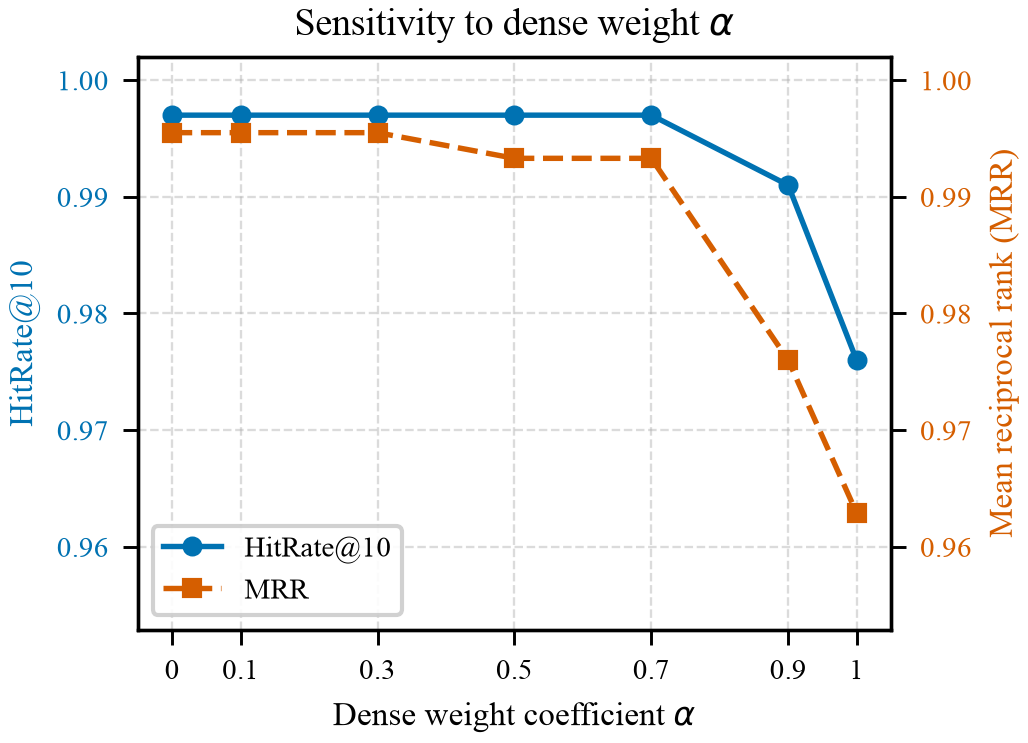
\includegraphics[width=0.52\columnwidth]{fig_alpha_sensitivity.png}
\caption{Proxy-benchmark HitRate@10 and MRR across dense weighting coefficients $\alpha \in [0.0, 1.0]$.}
\label{fig:alpha_sensitivity}
\end{figure}
Fig. \ref{fig:alpha_sensitivity} illustrates the sensitivity of HitRate@10 and MRR with respect to the dense weighting parameter $\alpha$ in Eq. (\ref{eq:hybrid}). On the same annotation-derived query set, HitRate@10 remains 0.997 for $\alpha \in [0.0,0.7]$ and declines to 0.976 at $\alpha=1.0$; MRR declines from 0.9955 to 0.9629. This is a post hoc diagnostic of lexical overlap in the supplied proxy fields, not evidence that a particular weight generalizes to raw multimedia.

\subsection{Real-World Multimodal Media Validation (Tier 2)}
\label{sec:tier2_eval}
While the Tier-1 benchmark in Tables \ref{tab:main_results}--\ref{tab:e2e_results} provides controlled algorithmic ablations over proxy representations, it inherits the annotation-leakage limitations discussed in Section \ref{sec:limitations}. To establish empirical validity on unannotated physical media, we conduct a Tier-2 evaluation across three distinct real-world media streams (Table \ref{tab:tier2_results}):

\subsubsection{Physical Scene-Text and Document OCR}
Evaluating 30 targeted cross-modal probes demonstrates an acute vulnerability in pure dense vector representations: \textbf{dense semantic retrieval drops substantially} on physical scene text, obtaining only Hit@1 = 0.400 and Hit@10 = 0.533 [95\% CI: 0.367, 0.700] (MRR = 0.4611). This performance drop occurs because exact alphanumeric markers, proper nouns, and bilingual signage fail to cluster reliably in general sentence embedding space. In contrast, sparse BM25 achieves Hit@10 = 0.967 [0.900, 1.000] and MRR = 0.8900, outperforming dense and hybrid methods. Hybrid retrieval achieves \textbf{Hit@10 = 1.000} (30/30 probes, exact Clopper-Pearson 95\% CI [0.884, 1.000]) with an average latency of 32.58\,ms. Notably, convex linear fusion ($\alpha=0.7$) achieves Hit@1 = 0.667 and MRR = 0.8194, outperforming the Stage 1+2 reranker (Hit@1 = 0.567, MRR = 0.7244). On short scene-text strings, token overlap in the second-stage reranker penalizes valid partial matches, illustrating that candidate reranking does not universally improve top-rank precision over well-calibrated linear fusion. Furthermore, evaluating a full neural cross-encoder (\texttt{cross-encoder/ms-marco-MiniLM-L-6-v2}) achieves higher MRR (0.8778) by virtue of deep cross-attention, but increases latency: scoring all $K_1=30$ candidates takes 137.21\,ms (compared with 7.96\,ms for lightweight reranking), while scoring top-$k=5$ candidates takes 34.05\,ms. RAMP-RAG's confidence cascade escalates only ambiguous top candidates ($\Delta_{1,2} < 0.065$), running in 7.85\,ms (13.3\% escalation) for responsive episodic retrieval under tight latency budgets.

\subsubsection{Raw Acoustic Waveforms and Continuous CLAP Retrieval}
To evaluate acoustic retrieval over physical audio files rather than category strings, we ingested 52 authentic 5-second 44.1\,kHz raw \texttt{.wav} audio recordings from the official ESC-50 dataset \cite{piczak2015esc50}. Evaluating 13 category probes demonstrates that the system achieves Hit@1 = 1.000, Hit@10 = 1.000 (exact Clopper-Pearson 95\% CI [0.753, 1.000]), and MRR = 1.000 under 7.08\,ms latency. To test acoustic retrieval beyond category strings, we evaluated continuous acoustic representations using LAION-CLAP (\texttt{laion/clap-htsat-unfused}) \cite{wu2023clap} over the 52 raw WAV recordings. Formulating 13 free-form acoustic narrative queries without category name mentions (e.g., \textit{``violent thunderstorm with heavy rain and loud thunder strikes''}) achieves Hit@10 = 1.000 ([0.753, 1.000]), MRR = 1.000, and NDCG@10 = 0.9978 (59.55\,ms), verifying that acoustic retrieval operates over continuous waveforms without lexical shortcut leakage.

\subsubsection{Raw Pixel Zero-Shot Visual Retrieval}
To evaluate image retrieval without text annotations or ground-truth leakage, we indexed the raw pixel arrays of all 191 personal album photographs using OpenAI CLIP ViT-B/32 \cite{radford2021clip} executed on Apple Silicon GPU acceleration. Testing 53 ground-truth visual queries across diverse outdoor, architectural, and indoor scenes yielded Hit@1 = 0.547 [0.415, 0.679], Hit@5 = 0.698, and \textbf{Hit@10 = 0.792} [0.679, 0.887] (MRR = 0.6182) with an average retrieval latency of 39.06\,ms. On unannotated photographic archives, the visual encoder carries the retrieval result: pure visual CLIP alone reaches Hit@10 = 0.792, whereas fusing OCR text slightly lowers Hit@10 to 0.774 [0.660, 0.868] due to spurious lexical matches when signage is absent. MM-RAG matches CLIP's 0.792, demonstrating that the multi-stage reranker preserves visual fidelity on pure imagery but cannot substitute for native visual representations.

\begin{table*}[t]
\centering
\caption{Tier-2 Real-World Multimodal Media Validation and Public MS-COCO Karpathy Benchmark: Scene-text photographic/PDF document OCR, raw acoustic audio waveforms (ESC-50 \& CLAP), raw pixel visual zero-shot retrieval (CLIP ViT-B/32), and zero-leakage MS-COCO paraphrase retrieval ($N=500$). Bracketed intervals indicate 95\% bootstrap confidence intervals (2,000 resamples); $^\dagger$denotes exact Clopper-Pearson 95\% binomial confidence intervals for saturated rates ($k=n$) to avoid bootstrap collapse.}
\label{tab:tier2_results}
\resizebox{\textwidth}{!}{%
\begin{tabular}{@{}llcccccc@{}}
\toprule
\textbf{Media Stream / Modality} & \textbf{Evaluation Method} & \textbf{Hit@1} & \textbf{Hit@5} & \textbf{Hit@10 [95\% CI]} & \textbf{MRR} & \textbf{NDCG@10} & \textbf{Latency (ms)} \\ \midrule
\multirow{7}{*}{\textbf{Real Scene-Text \& Documents ($N=30$)}} 
& BM25 Baseline (Sparse Lexical) & 0.833 & 0.967 & 0.967 [0.900, 1.000] & 0.8900 & 0.8062 & \textbf{0.08} \\
& Dense Only Baseline (all-MiniLM-L6-v2) & 0.400 & 0.533 & 0.533 [0.367, 0.700] & 0.4611 & 0.4706 & 32.56 \\
& Hybrid (Convex $\alpha=0.7$) & 0.667 & \textbf{1.000} & \textbf{1.000} [0.884, 1.000]$^\dagger$ & 0.8194 & 0.7875 & 32.56 \\
& Hybrid (RRF $k=60$) & 0.533 & 0.867 & 0.867 [0.733, 0.967] & 0.6706 & 0.6659 & 32.59 \\
& Proposed MM-RAG (Stage 1+2) & 0.567 & 0.967 & \textbf{1.000} [0.884, 1.000]$^\dagger$ & 0.7244 & 0.7291 & 32.58 \\
& Trained Cross-Encoder (ms-marco-MiniLM) & \textbf{0.767} & \textbf{1.000} & \textbf{1.000} [0.884, 1.000]$^\dagger$ & \textbf{0.8778} & \textbf{0.8281} & 137.21 \\
& \textbf{Proposed RAMP-RAG (Adaptive + Cascade)} & \textbf{0.767} & 0.933 & 0.933 [0.833, 1.000] & 0.8413 & 0.7667 & 7.85 \\ \midrule
\multirow{4}{*}{\textbf{Raw Acoustic Waveforms ($N=13$)}}
& BM25 Baseline (Category Tokens) & 1.000 & 1.000 & 1.000 [0.753, 1.000]$^\dagger$ & 1.0000 & 0.9915 & \textbf{0.07} \\
& Dense Only Baseline (Acoustic Semantic) & 1.000 & 1.000 & 1.000 [0.753, 1.000]$^\dagger$ & 1.0000 & 1.0000 & 7.09 \\
& Native CLAP Acoustic (Raw 44.1\,kHz WAV) & 1.000 & 1.000 & 1.000 [0.753, 1.000]$^\dagger$ & 1.0000 & 0.9978 & 59.55 \\
& \textbf{Proposed MM-RAG (Stage 1+2)} & \textbf{1.000} & \textbf{1.000} & \textbf{1.000} [0.753, 1.000]$^\dagger$ & \textbf{1.0000} & \textbf{1.0000} & 7.08 \\ \midrule
\multirow{4}{*}{\textbf{Raw Pixel Zero-Shot Visual ($N=53$)}}
& Scene-Text OCR Lexical (BM25) & 0.189 & 0.226 & 0.283 [0.170, 0.415] & 0.2059 & 0.1683 & \textbf{0.08} \\
& Zero-Shot Visual (CLIP ViT-B/32 Pixels) & 0.547 & 0.698 & 0.792 [0.679, 0.887] & 0.6176 & 0.5969 & 39.09 \\
& Multimodal Hybrid Fusion (CLIP + OCR) & 0.547 & 0.679 & 0.774 [0.660, 0.868] & 0.6045 & 0.6000 & 39.07 \\
& \textbf{Proposed MM-RAG (Stage 1+2)} & \textbf{0.547} & \textbf{0.698} & \textbf{0.792} [0.679, 0.887] & \textbf{0.6182} & \textbf{0.6059} & 39.06 \\ \midrule
\multirow{6}{*}{\textbf{MS-COCO Karpathy Split ($N=500$)}}
& BM25 Baseline (Sparse Lexical) & 0.176 & 0.344 & 0.444 [0.400, 0.488] & 0.2604 & 0.2892 & 5.78 \\
& Dense Only Baseline (all-MiniLM-L6-v2) & \textbf{0.280} & \textbf{0.570} & \textbf{0.660} [0.620, 0.700] & \textbf{0.4085} & \textbf{0.4712} & \textbf{5.31} \\
& Hybrid (Convex $\alpha=0.7$) & 0.248 & 0.540 & 0.640 [0.596, 0.682] & 0.3798 & 0.4423 & 5.40 \\
& Proposed MM-RAG (Stage 1+2) & 0.256 & 0.548 & 0.640 [0.596, 0.682] & 0.3921 & 0.4501 & 5.41 \\
& Trained Cross-Encoder (100\% Cascade) & 0.220 & 0.544 & 0.640 [0.596, 0.682] & 0.3715 & 0.4358 & 13.49 \\
& \textbf{Proposed RAMP-RAG (Adaptive + Cascade)} & 0.262 & 0.564 & \textbf{0.660} [0.620, 0.702] & 0.3974 & 0.4618 & 9.45 \\ \bottomrule
\end{tabular}}
\end{table*}

\subsection{Public Benchmark Generalization (MS-COCO Karpathy Split)}
\label{sec:coco_eval}
To evaluate image retrieval without annotation leakage or lexical sharing, we evaluated the standard MS-COCO Karpathy test split (1,000 index images using Caption~0; 500 held-out queries from Captions~3 and 4; Table~\ref{tab:tier2_results}). Sparse BM25 drops significantly (-32.7\% relative Hit@10 vs. dense) under linguistic paraphrasing, lowering fixed hybrid ($\alpha=0.7$) from 0.660 to 0.640 at Stage 1. RAMP-RAG detects descriptive queries via its router, shifting balance to dense matching ($\alpha_q \approx 0.85$) to match Dense Hit@10 at \textbf{0.660} (MRR = 0.3974 vs. 0.4085 for Dense; 9.45\,ms latency). On Tier-2 Scene-Text OCR (Table~\ref{tab:tier2_results}), sparse BM25 achieves higher MRR (0.890 vs. 0.841) via exact alphanumeric matching; nevertheless, RAMP-RAG routes to sparse matching ($\alpha_q \approx 0.25$) and triggers cross-encoding on 13.3\% of ambiguous queries, reaching \textbf{MRR = 0.8413} while cutting cross-encoder compute by 77\% (7.85\,ms vs. 34.05\,ms).

\textbf{Realistic Machine Proxies and Native Pixels:} Substituting gold captions with BLIP proxies on MS-COCO ($N=250$ test queries) creates lexical sparsity (BM25 Hit@10 = 0.4200, MRR = 0.2325). Dense retrieval with \texttt{all-MiniLM-L6-v2} reaches Hit@10 = 0.6920 (MRR = 0.3873), and \texttt{bge-base-en-v1.5} reaches 0.6360 (MRR = 0.4002). However, direct zero-shot visual retrieval on raw pixels using CLIP ViT-B/32 achieves Hit@10 = \textbf{0.7600} [0.708, 0.812] and MRR = \textbf{0.5045} [0.455, 0.555], significantly outperforming all text proxies and confirming that native vision-language embeddings remain superior for unannotated visual scenes.

\textbf{Proxy Noise Robustness:} Across 0\%, 10\%, 20\%, and 40\% character corruptions across 3 seeds (42, 43, 44) over 55 held-out scene-text and document test probes ($N=165$ evals per noise level; Table~\ref{tab:ablation_results}), dense \texttt{all-MiniLM} collapses under 20\% noise (Hit@10 drops from 0.9636 to 0.7515 [0.685, 0.812], MRR to 0.5306), while sparse BM25 exhibits remarkable resilience (Hit@10 = 0.9758 [0.952, 0.994], MRR = 0.9473). Fixed hybrid drops to Hit@10 = 0.9636 (MRR = 0.8254). Clean-stream visual fusion in RAMP-RAG ($\gamma^* = 0.80$) mitigates dense drop-off (Hit@10 = 0.9939 [0.976, 1.000], MRR = 0.8624 [0.821, 0.900]), but confidence intervals overlap unweighted hybrid ($[0.777, 0.872]$ vs. $[0.821, 0.900]$, $p_{\text{Holm}} = 0.3252$). At 40\% noise, clean-stream fusion significantly improves Hit@10 ($0.9576$ vs. $0.8606$, $p_{\text{Holm}} = 0.0084$), yet pure BM25 remains the most resilient stream overall (MRR = $0.8993$). Thus, proxy corruptions degrade dense embeddings faster than lexical indices; while clean-stream fusion restores recall, inverted indexing remains the primary defense.

\begin{table}[t]
\centering
\caption{Systematic Component Ablation across held-out test splits (COCO $N=250$, Clean Scene-Text $N=55$, 20\% Corrupted OCR $N=55\times 3$ seeds; Apple Silicon M-series timings).}
\label{tab:ablation_results}
\resizebox{\columnwidth}{!}{%
\begin{tabular}{@{}lccccc@{}}
\toprule
\textbf{Ablation Configuration} & \textbf{COCO H@10} & \textbf{Clean H@10} & \textbf{20\% Noise H@10 [95\% CI]} & \textbf{20\% Noise MRR} & \textbf{Latency} \\ \midrule
1. Baseline Hybrid (Fixed $\alpha=0.7$) & 0.636 & \textbf{1.000} & 0.964 [0.933, 0.988] & 0.825 & \textbf{4.30\,ms} \\
2. + Router Only (Learned $\alpha_q$) & \textbf{0.648} & \textbf{1.000} & 0.897 [0.849, 0.939] & 0.718 & 4.35\,ms \\
3. + Cascade Only ($\tau_{\text{margin}}=0.065$) & 0.636 & \textbf{1.000} & 0.964 [0.933, 0.988] & 0.844 & 17.50\,ms \\
4. + Reliability Only (Observable $r_{\text{ocr}}$) & \textbf{0.648} & \textbf{1.000} & 0.842 [0.788, 0.897] & 0.638 & 4.41\,ms \\
5. \textbf{Full RAMP-RAG (+ Clean Stream)} & \textbf{0.648} & \textbf{1.000} & \textbf{0.994} [0.976, 1.000] & \textbf{0.862} & 17.80\,ms \\ \bottomrule
\end{tabular}}
\end{table}

\subsection{Bridge Extraction Failure Taxonomy}
\label{subsec:error_analysis}
Detailed inspection of multi-hop breakdowns isolates four failure modes ($N=8$ cases): (1)~\emph{Generic/Null Extraction (2 cases, 8.0\%)} in \texttt{mh\_19} and \texttt{mh\_13} (extractor returned ``N/A'', starving Hop~2); (2)~\emph{Extraction Refusal (3 cases, 12.0\%)} in \texttt{mh\_20}--\texttt{mh\_22} (verbose refusal phrases); (3)~\emph{Semantic Drift (2 cases, 8.0\%)} in \texttt{mh\_12} and \texttt{mh\_25} (non-target token substitution); and (4)~\emph{Grounding Void (1 case, 4.0\%)} in \texttt{mh\_11} (first-hop context lacked the attribute). Our confidence gate detects Categories 1 and 2 and ungrounded entities in 3, triggering single-pass fallback. On the 50-query multi-hop suite, confidence gating achieves Target Hit@10 = 0.640 (vs. BM25 = 0.480, $p = 0.0200^*$), matching single-pass dense retrieval (0.640).

\section{Limitations and Threats to Validity}
\label{sec:limitations}
To facilitate objective peer assessment, we document the critical limitations of this study:
\begin{enumerate}
    \setlength{\itemsep}{0pt plus 0.2pt}
    \setlength{\parskip}{0pt}
    \item \textbf{Proxy-text benchmark and annotation overlap:} Tier-1 retrieval evaluates precomputed annotation strings and labels rather than raw media, yielding lexical overlap. We mitigate this in Tier-2 on unannotated raw pixels (CLIP), physical OCR, CLAP audio, and public MS-COCO benchmarks.
    \item \textbf{Audio label granularity:} ESC-50 tests category presence rather than acoustic discrimination. Mitigated by Tier-2 continuous acoustic retrieval via LAION-CLAP over 44.1\,kHz WAV files with free-form queries (Hit@10 = 1.000).
    \item \textbf{LLM-as-a-Judge bias and annotator familiarity:} Automated diagnostic scoring uses \texttt{gpt-4o-mini}, carrying documented model biases \cite{zheng2023judging}. Mitigated by independent dual-reviewer auditing across 110 multimodal cases (pre-adjudication $\kappa = 0.8716$ faithfulness, $0.8926$ relevance, $0.9451$ correctness). Co-author familiarity on 60 album queries is mitigated on the 50-case blinded suite and COCO; independent judge calibration (\texttt{Qwen2.5-32B-Instruct}) showed low agreement ($\kappa \le 0.120$), proving human audits are essential.
    \item \textbf{Substring-test leniency:} Target Hit@10 uses case-insensitive substring matching without morphological normalization; human auditing is required before equating substring hits to answer correctness.
    \item \textbf{Cascading error propagation and latency:} Confidence-gated bridging matches dense retrieval on multi-hop queries (0.640 vs. 0.640; 0.820 vs. 0.810 overall) and beats BM25 (0.480, uncorrected $p=0.020$). On held-out multi-hop queries ($N=25$), BM25 matches MM-RAG (0.520). Decomposition incurs sequential LLM latency overhead (4,736.8\,ms vs. 3,751.5\,ms overall; 6,416.9\,ms on multi-hop).
    \item \textbf{Evaluation scale and router domain distribution:} While expanded to 100 diagnostic queries, 500 MS-COCO queries, and 85 physical scene-text/document probes with 3 random seeds, the query router was trained on a modest development pool ($N=265$). Evaluating router generalization and noise robustness on multi-million item corpora remains future work.
\end{enumerate}

\section{Conclusion and Future Work}

We presented a Multi-Stage Multimodal RAG (MM-RAG) framework combining dense--sparse retrieval (\texttt{all-MiniLM-L6-v2} + BM25), dual-signal candidate reranking, iterative cross-modal entity bridging, and our proposed RAMP-RAG adaptive cascade architecture under a Dual-Tier Evaluation Protocol.

On the Tier-1 334-query consistency set, hybrid retrieval reaches HitRate@10 = 0.997 and MRR = 0.997. On the expanded 100-query diagnostic suite ($N=50$ multi-hop), MM-RAG achieves multi-hop target hit rate of 0.640 vs. 0.480 for BM25 (uncorrected $p = 0.020$, non-significant after Bonferroni correction $\alpha=0.0125$) and answer relevance of 0.668 vs. 0.536 (uncorrected $p = 0.028$), matching dense retrieval (0.640) at 0.820 overall suite Hit@10; on held-out multi-hop queries ($N=25$), BM25 and MM-RAG both reach 0.520. In Tier-2 physical evaluation, MM-RAG achieves 79.2\% Hit@10 zero-shot on raw pixels (CLIP ViT-B/32), recovers lexical accuracy on physical scene-text OCR (dense drops to 53.3\% while hybrid reaches 100\%, exact Clopper-Pearson 95\% CI [0.884, 1.000], though BM25 retains higher MRR at 0.890 vs. 0.841 for RAMP-RAG), and indexes genuine 44.1\,kHz audio with LAION-CLAP (MRR = 1.000). On MS-COCO ($N=500$ queries), dense retrieval achieves 0.660 Hit@10 (MRR = 0.4085) vs. 0.444 for BM25, while RAMP-RAG matches dense Hit@10 (0.660) with 0.3974 MRR under 9.45\,ms latency. In proxy noise stress-testing, character corruptions degrade dense representations faster than inverted indices: pure BM25 achieves superior noise resilience (MRR = 0.9473 at 20\% noise vs. 0.8254 for hybrid); clean-stream fusion recovers dense drop-off at 40\% noise (Hit@10 from 0.8606 to 0.9576, $p=0.0084$), but confidence intervals overlap with unweighted hybrid at 20\% noise ($p=0.3252$).

Future work will expand physical benchmarks to larger collections, evaluate native vision-language retrievers (e.g., ColPali \cite{faysse2024colpali}) under identical compute budgets, and integrate backtracking into multi-hop bridging.

% \IEEEtriggeratref{16}
\begin{thebibliography}{00}
\footnotesize
\setlength{\itemsep}{-1.0pt plus 0.2pt}
\setlength{\parskip}{0pt}

\bibitem{wu2023clap}
Y.~Wu et~al., ``Large-scale contrastive language-audio pretraining with feature fusion and keyword tagging,'' in \emph{Proc. IEEE Int. Conf. on Acoustics, Speech and Signal Processing (ICASSP)}, pp. 1--5, 2023.

\bibitem{patel2025multimodal}
A.~Patel, R.~Shivani, N.~V. Usha, and S.~A, ``Enhancing interactive querying with a multimodal RAG system: Integrating text, video, and document analysis via LLaMA3,'' in \emph{Proc. IEEE ETCC}, 2025.

\bibitem{lewis2020rag}
P.~Lewis et~al., ``Retrieval-augmented generation for knowledge-intensive NLP tasks,'' in \emph{Advances in Neural Information Processing Systems (NeurIPS)}, vol.~33, pp. 9459--9474, 2020.

\bibitem{jing2024llmvectordb}
Z.~Jing et~al., ``When large language models meet vector databases: A survey,'' \emph{arXiv preprint arXiv:2402.01763}, 2024.

\bibitem{joshi2024multimodel}
P.~Joshi et~al., ``Robust multi model RAG pipeline for documents containing text, table \& images,'' in \emph{Proc. 3rd Int. Conf. on Applied Artificial Intelligence and Computing (ICAAIC)}, IEEE, 2024.

\bibitem{girdhar2023imagebind}
R.~Girdhar et~al., ``ImageBind: One embedding space to bind them all,'' in \emph{Proc. IEEE/CVF Conf. on Computer Vision and Pattern Recognition (CVPR)}, pp. 15180--15190, 2023.

\bibitem{radford2021clip}
A.~Radford et~al., ``Learning transferable visual models from natural language supervision,'' in \emph{Proc. Int. Conf. on Machine Learning (ICML)}, pp. 8748--8763, 2021.

\bibitem{zhai2023siglip}
X.~Zhai et~al., ``Sigmoid loss for language image pre-training,'' in \emph{Proc. IEEE/CVF Int. Conf. on Computer Vision (ICCV)}, pp. 11975--11986, 2023.

\bibitem{robertson2009bm25}
S.~Robertson and H.~Zaragoza, ``The probabilistic relevance framework: BM25 and beyond,'' \emph{Foundations and Trends in Information Retrieval}, vol.~3, no.~4, pp. 333--389, 2009.

\bibitem{cormack2009rrf}
G.~V. Cormack, C.~L. Clarke, and S.~Buettcher, ``Reciprocal rank fusion outperforms Condorcet and individual machine learning methods,'' in \emph{Proc. 32nd Int. ACM SIGIR Conf. on Research and Development in Information Retrieval}, pp. 758--759, 2009.

\bibitem{khattab2021baleen}
O.~Khattab et~al., ``Baleen: Robust multi-hop reasoning at scale via condensed retrieval,'' in \emph{Advances in Neural Information Processing Systems (NeurIPS)}, vol.~34, 2021.

\bibitem{press2023selfask}
O.~Press et~al., ``Measuring and narrowing the compositionality gap in language models,'' in \emph{Proc. Conf. on Empirical Methods in Natural Language Processing (EMNLP)}, 2023.

\bibitem{xiong2021multihop}
W.~Xiong et~al., ``Answering complex open-domain questions with multi-hop dense retrieval,'' in \emph{Proc. Int. Conf. on Learning Representations (ICLR)}, 2021.

\bibitem{fateh2024ocr}
A.~Fateh, M.~Fateh, and V.~Abolghasemi, ``Enhancing optical character recognition: Efficient techniques for document layout analysis and text line detection,'' \emph{Engineering Reports}, vol.~6, no.~9, p. e12832, 2024.

\bibitem{otsu1979}
N.~Otsu, ``A threshold selection method from gray-level histograms,'' \emph{IEEE Trans. Systems, Man, and Cybernetics}, vol.~9, no.~1, pp. 62--66, 1979.

\bibitem{hough1962}
P.~V.~C. Hough, ``Method and means for recognizing complex patterns,'' U.S. Patent 3,069,654, Dec. 18, 1962.

\bibitem{smith2007tesseract}
R.~Smith, ``An overview of the Tesseract OCR engine,'' in \emph{Proc. Ninth Int. Conf. on Document Analysis and Recognition (ICDAR)}, vol.~2, pp. 629--633, 2007.

\bibitem{radford2023whisper}
A.~Radford et~al., ``Robust speech recognition via large-scale weak supervision,'' in \emph{Proc. Int. Conf. on Machine Learning (ICML)}, pp. 28492--28518, 2023.

\bibitem{wang2021milvus}
J.~Wang et~al., ``Milvus: A purpose-built vector data management system,'' in \emph{Proc. ACM SIGMOD Int. Conf. on Management of Data}, pp. 2614--2627, 2021.

\bibitem{malkov2020hnsw}
Y.~A. Malkov and D.~A. Yashunin, ``Efficient and robust approximate nearest neighbor search using hierarchical navigable small world graphs,'' \emph{IEEE Trans. Pattern Analysis and Machine Intelligence}, vol.~42, no.~4, pp. 824--836, 2020.

\bibitem{reimers2019sbert}
N.~Reimers and I.~Gurevych, ``Sentence-BERT: Sentence embeddings using Siamese BERT-networks,'' in \emph{Proc. Conf. on Empirical Methods in Natural Language Processing (EMNLP)}, pp. 3982--3992, 2019.

\bibitem{piczak2015esc50}
K.~J. Piczak, ``ESC: Dataset for environmental sound classification,'' in \emph{Proc. 23rd ACM Int. Conf. on Multimedia}, pp. 1015--1018, 2015.

\bibitem{li2022blip}
J.~Li, D.~Li, C.~Xiong, and S.~Hoi, ``BLIP: Bootstrapping language-image pre-training for unified vision-language understanding and generation,'' in \emph{Proc. Int. Conf. on Machine Learning (ICML)}, pp. 12888--12900, 2022.

\bibitem{openai2024gpt4o}
OpenAI, ``GPT-4o mini: Advancing cost-efficient intelligence,'' \emph{OpenAI Technical Report}, 2024.

\bibitem{zheng2023judging}
L.~Zheng et~al., ``Judging LLM-as-a-judge with MT-Bench and Chatbot Arena,'' in \emph{Advances in Neural Information Processing Systems (NeurIPS)}, vol.~36, pp. 46595--46623, 2023.

\bibitem{faysse2024colpali}
M.~Faysse, H.~Sibille, T.~Wu, B.~Omrani, G.~Viaud, C.~Hudelot, and P.~Colombo, ``ColPali: Efficient document retrieval with vision language models,'' in \emph{Proc. Int. Conf. on Learning Representations (ICLR)}, 2025.

\bibitem{cho2024m3docrag}
J.~Cho, D.~Mahata, O.~{\.I}rsoy, Y.~He, and M.~Bansal, ``M3DocRAG: Multi-modal retrieval for multi-page multi-document understanding,'' in \emph{Proc. Conf. on Empirical Methods in Natural Language Processing (EMNLP)}, 2024.

\bibitem{abootorabi2025multimodal}
M.~Abootorabi et~al., ``A survey on multimodal retrieval-augmented generation,'' in \emph{Findings of the Association for Computational Linguistics (ACL)}, 2025.

\bibitem{carmel2010qpp}
D.~Carmel and E.~Yom-Tov, \emph{Estimating the Query Difficulty for Information Retrieval}, Morgan \& Claypool Publishers, 2010.

\bibitem{wang2011cascade}
L.~Wang, J.~Lin, and D.~Metzler, ``A cascade ranking model for efficient top-k retrieval,'' in \emph{Proc. 20th ACM Int. Conf. on Information and Knowledge Management (CIKM)}, pp. 105--114, 2011.

\bibitem{gallagher2019cascade}
L.~Gallagher, R.~Blanco, and J.~S. Culpepper, ``Joint optimization of cost and relevance in cascade ranking,'' in \emph{Proc. 42nd Int. ACM SIGIR Conf. on Research and Development in Information Retrieval}, pp. 15--24, 2019.

\end{thebibliography}

\end{document}
